%%%%%%%%%%%%%%%%%%%%%%%%%%%%%%%%%%%%%%%%%%%%%%%%%
\section{STOCHASTIC-GRADIENT LD} \label{sgld}
%%%%%%%%%%%%%%%%%%%%%%%%%%%%%%%%%%%%%%%%%%%%%%%%%
\begin{eqnarray}
  h & = & \frac{N}{n} \sum_{i=1}^n \nabla \log p(\bx_i | \thetav)- \sum_{i=1}^N \nabla \log p(\bx_i | \thetav ) \\
    & = & \frac{N}{n} \sum_{i=1}^n s_i \\
  s_i & = & \nabla \log p(\bx_i | \thetav) + \frac{1}{N} \nabla p(\thetav) \\
  \text{V}(h) & = & \frac{N^2}{n^2} \sum_{i=1}^n \text{Var}(s_i) \\
                & = & \frac{N^2}{n^2} \sum_{i=1}^n \frac{1}{n} \lp \sum_{j=1} (s_i - \bar{s})^2 \rp \\
                & = & \frac{N^2}{n^2} \sum_{i=1}^n V_s \\
                & = & \frac{N^2}{n^2} n V_s \\
                & = & \frac{N^2}{n} V_s 
  %\text{Var}(\thetav) & = & \frac{\epsilon^2}{4}\text{Var}(h) + \epsilon \\
  %       \frac{\epsilon^2}{4}\text{Var}(h) & << & \epsilon \\
  %       \frac{\epsilon N^2}{4 n} V_s & << & 1       
\end{eqnarray}
\begin{eqnarray}
  \text{Var}(\thetav) & = & \frac{\epsilon^2}{4}\text{Var}(h) + \epsilon \\
         \frac{\epsilon^2}{4}\text{Var}(h) & << & \epsilon \\
         \frac{\epsilon N^2}{4 n} V_s & << & 1       
\end{eqnarray}

%%%%%%%%%%%%%%%%%%%%%%%%%%%%%%%%%%%%%%%%%%%%%%%%%
\section{SGLD-ABC} \label{sgld}
%%%%%%%%%%%%%%%%%%%%%%%%%%%%%%%%%%%%%%%%%%%%%%%%%

\subsection{ABC Cost Function}



For optimization purposes we can search for the maximum a posteriori (MAP) estimator $\hat{\thetav}$ using the log-joint distribution $\hat{\thetav} = \argmax_{\thetav} \mathcal{MAP}$, where $\mathcal{MAP}$ is
\begin{eqnarray}
  \mathcal{LJ} &    =    & \log \pi(\thetav) + \log \pi\lp \y | \thetav \rp \\
                & \approx &\log \pi(\thetav) + \log \sum_{s=1}^S \pi_{\epsvec}\lp \y | f\lp \thetav, \omega_s \rp \rp - \log S
\end{eqnarray} 
we can also maximize the lower-bound of $\mathcal{LJ} \geq \mathcal{LB}$, where 
\begin{eqnarray}
  \mathcal{LB} & \approx &\log \pi(\thetav) + \sum_{s=1}^S \log  \pi_{\epsvec}\lp \y | f\lp \thetav, \omega_s \rp \rp
\end{eqnarray} 
which will be more convenient for optimization for typical kernels (i.e. $\pi_{\epsilon}$ is Gaussian).

The simplest optimization is to set the objective function  $C$ to be $-\mathcal{LJ}$ or $-\mathcal{LB}$ and compute stochastic gradients using 2SPSA with $q$ repeats (negative log-likelihood because we will assume minimization):
\begin{eqnarray}
  \frac{\partial C}{\partial \thetav} & = & \frac{1}{q} \sum_{j=1}^{q} \frac{C\lp \thetav + c \Delta_j\rp - C{\lp\thetav - c \Delta_j\rp}}{2 c \Delta_j}
\end{eqnarray}
or 1SPSA
\begin{eqnarray}
  \frac{\partial C}{\partial \thetav} & = & \frac{1}{q} \sum_{j=1}^{q}  \frac{C\lp \thetav + c \Delta_j\rp - C(\thetav)}{c \Delta_j}
\end{eqnarray}
which is less accurate but is less computation if $C(\thetav)$ is computed at each step (TODO: possible algorithm).  TODO: rewrite $\frac{\partial C}{\partial \thetav}$ as $\hat{g}$ or similar.

\subsection{Special Case: Gaussian Kernels}
When the kernel is known we can use the chain rule to compute the gradients with the first part from the kernel and the second from the variation of the simulator pseudo-statistics, whose gradient can be estimated using SPSA.  Expanding the likelihood over $J$ statistics, the lower bound on the loglikelihood becomes:
\begin{eqnarray}
  \hat{L} & = & \sum_s \log \pi_{\epsilon}\lp \y | f(\thetav, \omega_s)\rp \\
          & = & \sum_s \log \prod_{j=1}^J \pi_{\epsilon_j}\lp y_j | f_j(\thetav, \omega_s)\rp \\
          & = & \sum_s \sum_j \log  \pi_{\epsilon_j}\lp y_j | f_j(\thetav, \omega_s)\rp \\
          & = & \sum_s \sum_j -\frac{1}{2} \frac{\lp y_j - f_j(\thetav, \omega_s)\rp^2}{\epsilon_j^2} - Z_j \\
\end{eqnarray}

The gradient:
\begin{eqnarray} 
  \nabla \hat{L} & = & \sum_s \sum_j \frac{\lp y_j - f_j(\thetav, \omega_s)\rp}{\epsilon_j^2} \cdot \frac{\partial f_j(\thetav, \omega_s)}{\partial \thetav} \\
                 & = & \sum_s \sum_j e_{js} \nabla_{js}
\end{eqnarray}
The first part $e_{js}$ is analytic, the second part $\nabla_{js}$ requires estimation by 2SPSA:
\begin{eqnarray} 
  \hat{ \nabla }_{js}  & = & \frac{1}{q} \sum_{r=1}^q \frac{f_j(\thetav + c \Delta_r , \omega_s) - f_j(\thetav - c \Delta_r , \omega_s)}{2 c \Delta_r}
\end{eqnarray}
or 1SPSA
\begin{eqnarray} 
  \hat{ \nabla }_{js} & = & \frac{1}{q} \sum_{r=1}^q \frac{f_j(\thetav + c \Delta_r , \omega_s) - f_j(\thetav, \omega_s)}{c \Delta_r}
\end{eqnarray}
the benefit of 1SPSA in this case is that the first gradients  $e_{js}$ can be computed from $f_j(\thetav, \omega_s)$.



\section{Applying SGLD to ABC}

There are two main sources of randomness in the ABC gradient computation: the random perturbation mask and the random seed of the simulator model, which controls the simulator noise.  This noise can be eliminated by using common random numbers \cite{spall-crn}.  On the other hand, it is not clear that this is the best strategy, as the noise from the masks at a fixed seed may be higher than   

\begin{eqnarray}
  V_{\gradestimaterepeat{t}{\thetav_t}{j}} & = & \frac{1}{q-1} \sum_{j=1}^q (\gradestimaterepeat{t}{\thetav_t}{j} - \gradestimate{t}{\thetav_t})^2 \\
  V_{\gradestimate{t}{\thetav_t}} & = & \frac{1}{q-1} V_{\gradestimaterepeat{t}{\thetav_t}{j}} \\
  \frac{\epsilon^2}{4 }V_{\gradestimate{t}{\thetav_t}} & = & \frac{\epsilon^2}{4 q }V_{\gradestimaterepeat{t}{\thetav_t}{j}} \\
                                                       & << & \epsilon \\
                    \frac{\epsilon}{4 (q-1) }V_{\gradestimaterepeat{t}{\thetav_t}{j}}  & << & 1                                  
\end{eqnarray}

Check for $g(\thetav) + h(\thetav) + \eta$ that $h(\thetav) + \eta \approx \eta$

Also $\theta_{t+1} = \theta_t + \frac{\epsilon}{2}\gradestimate{t}{\thetav_t} + \sqrt{\epsilon}\mathcal{N}(0,1)$

\subsection{Statistical Tests for Gradients}

From Byrd:
\begin{eqnarray}
\frac{||V_{\gradestimaterepeat{t}{\thetav_t}{j}} ||_1}{q} & \leq r^2 || \hat{g}_t ||_2^2 \\
\hat{q} & = & \frac{||V_{\gradestimaterepeat{t}{\thetav_t}{j}} ||_1}{r^2 || \hat{g}_t ||_2^2}
\end{eqnarray}

TODO:
\begin{itemize}
  \item Check that $q$ gradients are normal.  Especially as $q$ increases.
  \item Merge Byrd's test for $\hat{q}$ and condition on SGLD-ABC.
  \item Variance check for increasing $q$ can also be used to stop optimization since the variance is less than the noise in the gradients.
\end{itemize}

% \subsection{SGD, AdaGrad, RMSProp, AdaM}
  
% \begin{itemize}
%   \item  Arguably the two most useful procedures in simulation-based science are optimization and Bayesian inference.
%   \item  Optimization can take the form of simple grid-search to sophisticated techniques like factorial design \cite{factorialdesign}, Bayesian experiment design \cite{bayesexpdesign}, (mention others).
%   \item Recently, Bayesian optimization techniques have shown success in optimizing very expensive black-box simulators \cite{bosuccess}.
%   \item Though gradients are not directly computable for simulators, they can be computed analytically by using finite differences (see \cite{kiefer1952}).  This quickly becomes infeasible for large $p$ problems.  There is however an alternative stochastic approximation algorithm by Spall \cite{spall1999} that requires only 2 simulation calls independent of $p$.
%   \item By using this approximation, gradient-based algorithms can be adopted for simulators: for optimization, using analogous stochastic gradient descent algorithms and for Bayesian inference using Langevin dynamics \cite{langevin}.
% \end{itemize}
%
% With our stochastic gradient in hand, we can make use of robust stochastic gradient rules, including recent advances from machine learning.
%
% \subsubsection{SGD}
% The basic update rule is at time $t$ for minimization is
% \begin{eqnarray}
%   \Delta\thetav & = & - \alpha_t \hat{g_t}
% \end{eqnarray}
% with conditions $\sum_{t=1}^{\infty} \alpha_t = \infty$ and $\sum_{t=1}^{\infty} \alpha_t^2 < \infty$ required for convergence.
% An additional momentum parameter $\beta_1$ can be added to improve convergence
% \begin{eqnarray}
%   \gmom & = & \beta_1 \gmom + (1-\beta_1)*\hat{g_t} \\
%   \Delta\thetav & = & - \alpha_t \gmom
% \end{eqnarray}
%
% \subsubsection{AdaGrad}
% AdaGrad uses the total cumulative element-wise square of the gradients to automatically both decrease $\alpha_t$ and scale the learning rates for each dimension:
% \begin{eqnarray}
%   \gmom    & = & \beta_1 \gmom + (1-\beta_1)*\hat{g_t} \\
%   \gsquare & = & \sum_{t'=1}^t \hat{g_t}^2 \\
%   \Delta\thetav & = & - \alpha_t \gmom / \sqrt{\gsquare}
% \end{eqnarray}
%
% \subsubsection{RMSProp}
% \begin{eqnarray}
%   \gmom    & = & \beta_1 \gmom + (1-\beta_1)*\hat{g_t} \\
%   \gsquare & = & \beta_2 \gsquare + (1-\beta_2)*\hat{g_t}^2 \\
%   \Delta\thetav & = & - \alpha_t \gmom / \sqrt{\gsquare}
% \end{eqnarray}
%
% \subsubsection{AdaM}
% \begin{eqnarray}
%   \gmom    & = & \beta_1 \gmom + (1-\beta_1)*\hat{g_t} \\
%   \gsquare & = & \beta_2 \gsquare + (1-\beta_2)*\hat{g_t}^2 \\
%   \gamma & = & \frac{ \sqrt{1-(1-\beta_2)^t}}{(1-(1-\beta_1)^t)} \\
%   \Delta\thetav & = & - \alpha_t \gamma \gmom / \sqrt{\gsquare}
% \end{eqnarray}


% %%%%%%%%%%%%%%%%%%%%%%%%%%%%%%%%%%%%%%%%%%%%%%%%%
% \section{EXPERIMENTS} \label{experiments}
% %%%%%%%%%%%%%%%%%%%%%%%%%%%%%%%%%%%%%%%%%%%%%%%%%

% \subsection{Logistic Regression with Stochastic Gradients}
%
% \subsection{Optimization of Blowfly Dynamics}
%
% \subsubsection{Using AdaM}
%
% \begin{figure}[h]
% \vspace{1in}
% 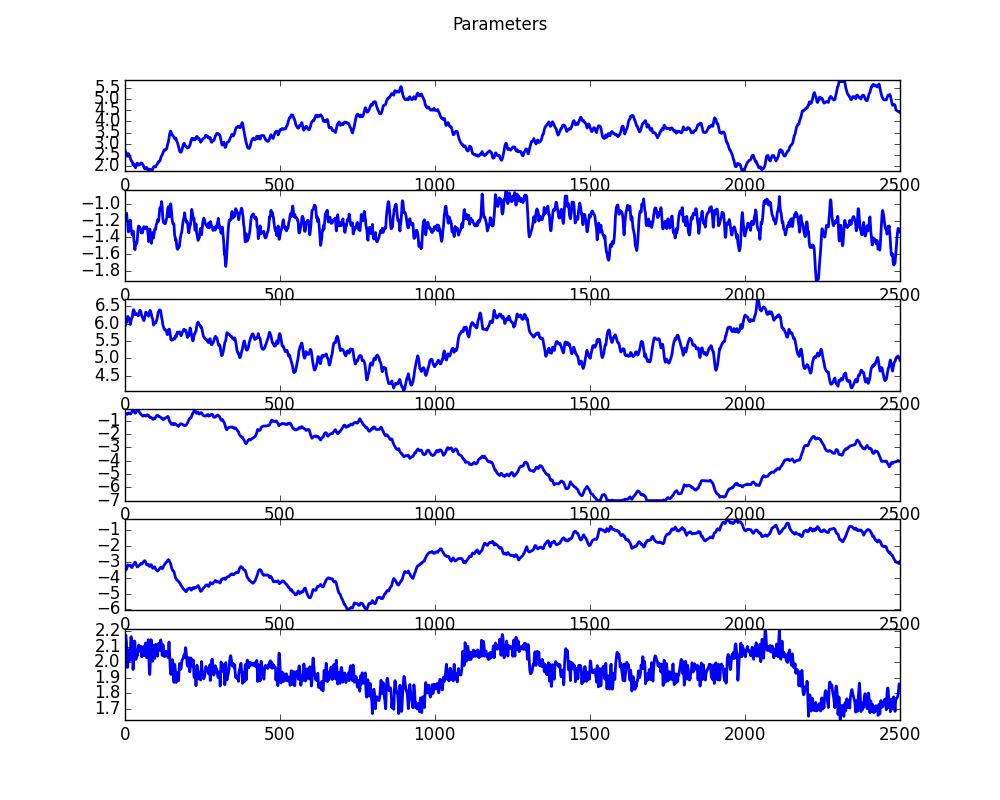
\includegraphics[width=0.45\columnwidth]{./images/blowfly_adam_post_series.png}
% 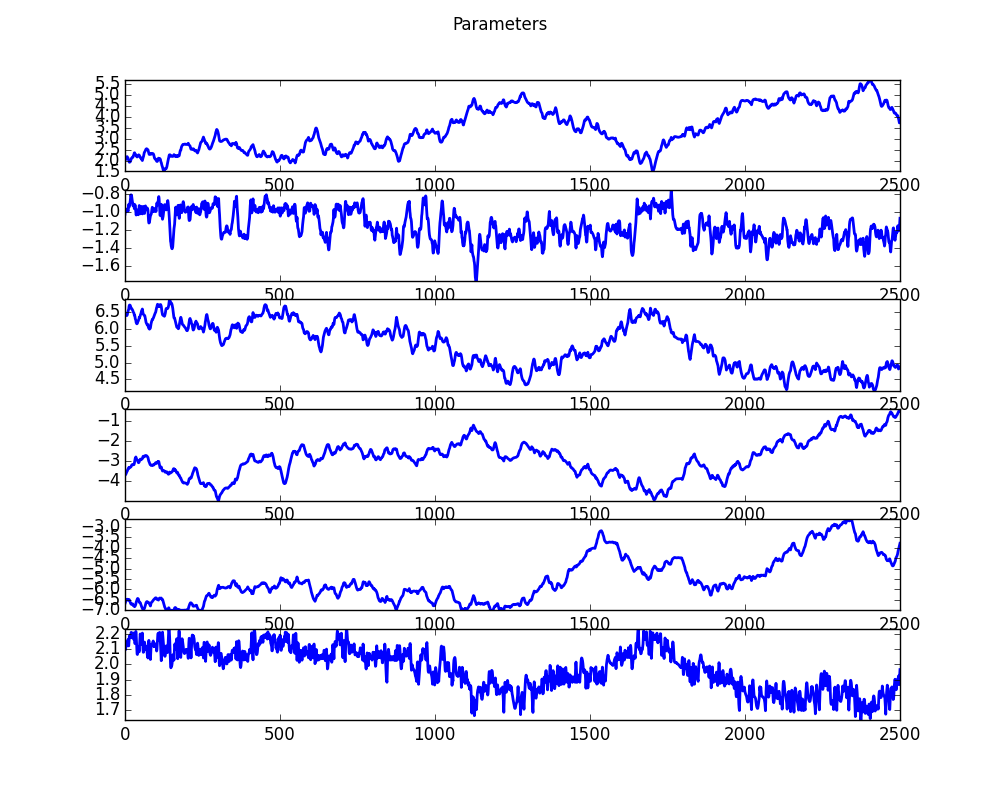
\includegraphics[width=0.45\columnwidth]{./images/blowfly_adam_post_series_sgld5k.png}
% 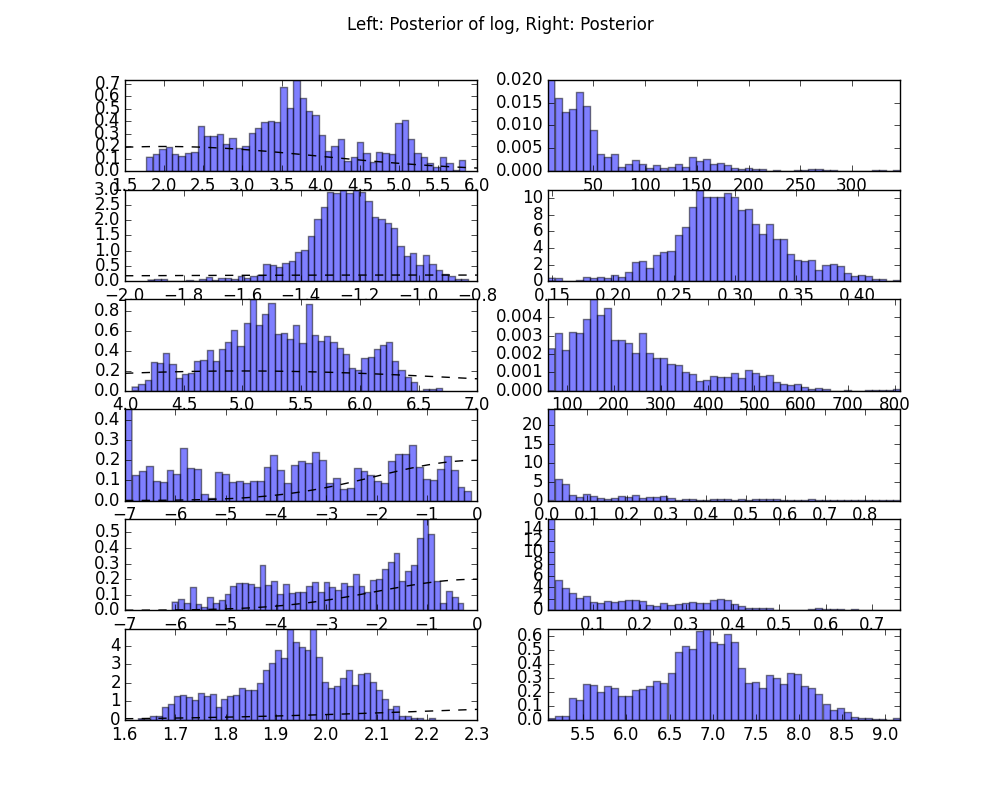
\includegraphics[width=0.45\columnwidth]{./images/blowfly_adam_post.png}
% 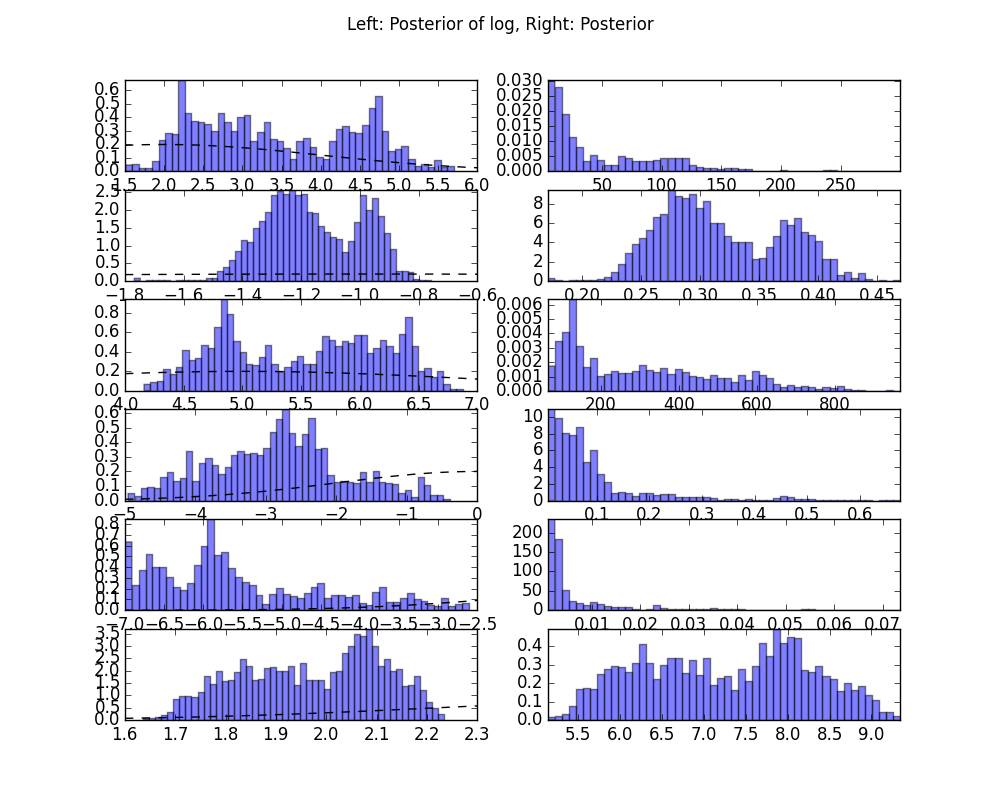
\includegraphics[width=0.45\columnwidth]{./images/blowfly_adam_post_sgld5k.png}
% 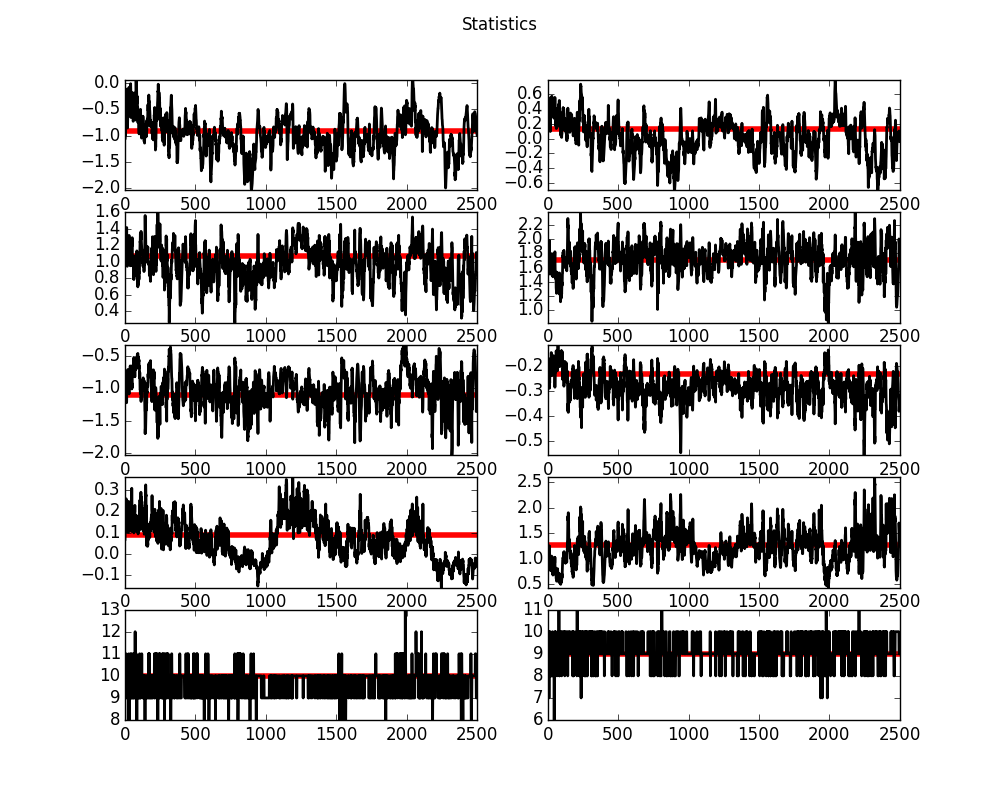
\includegraphics[width=0.45\columnwidth]{./images/blowfly_adam_postpred_series.png}
% 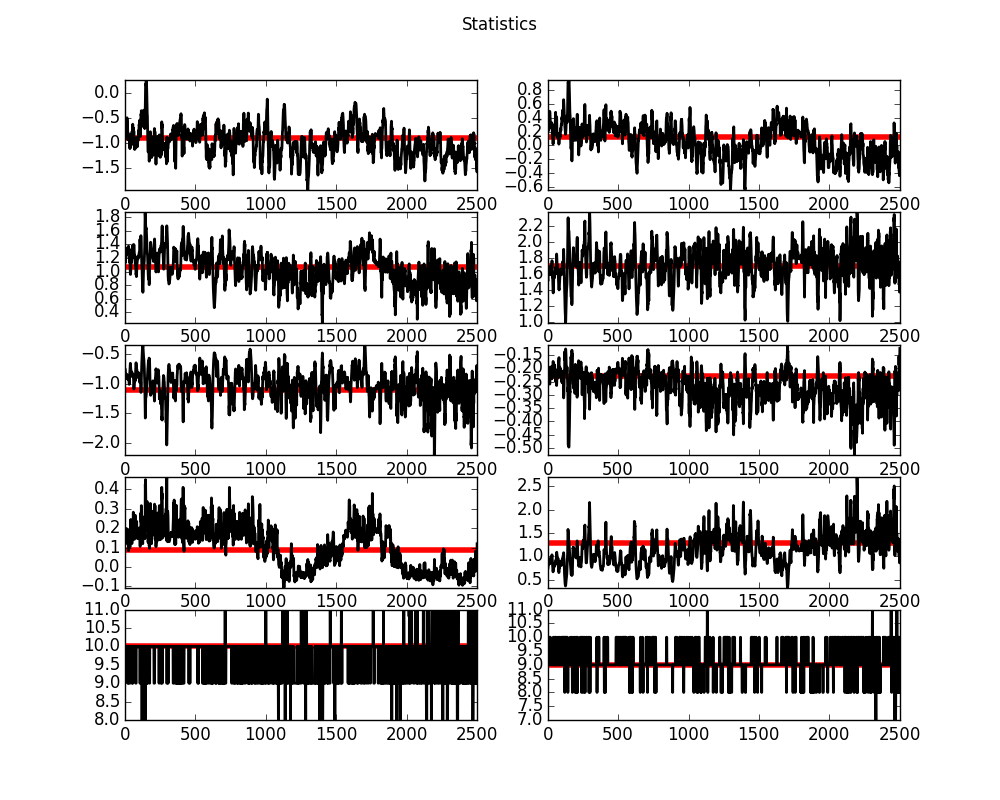
\includegraphics[width=0.45\columnwidth]{./images/blowfly_adam_postpred_series_sgld5k.png}
% 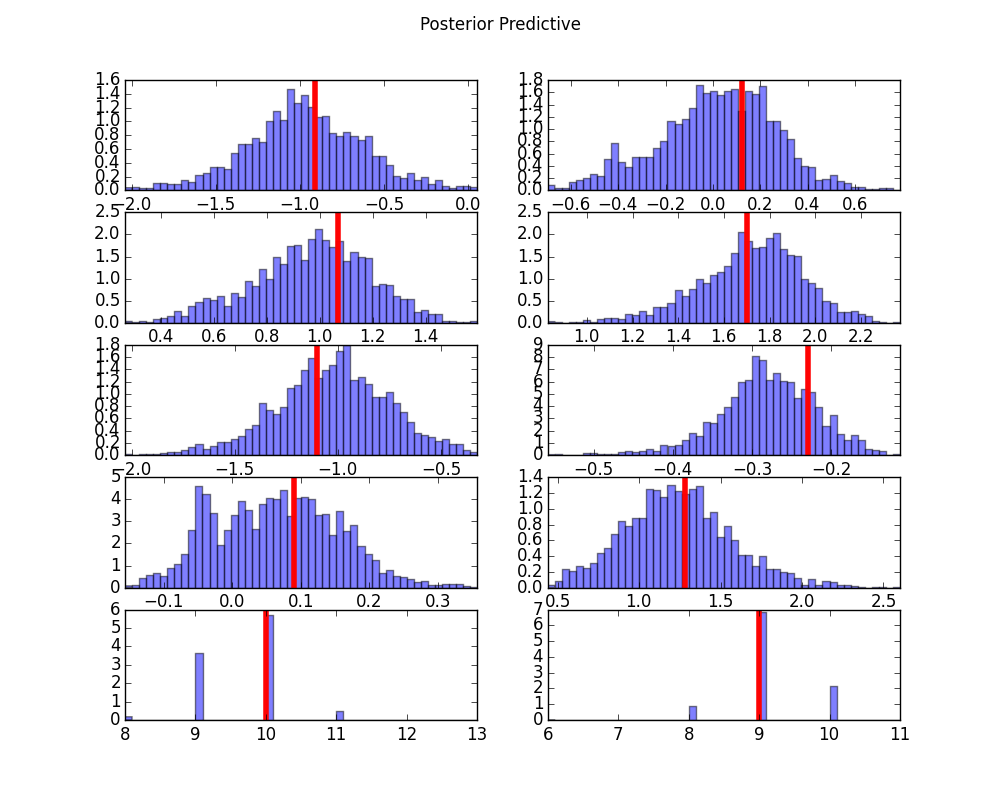
\includegraphics[width=0.45\columnwidth]{./images/blowfly_adam_postpred.png}
% 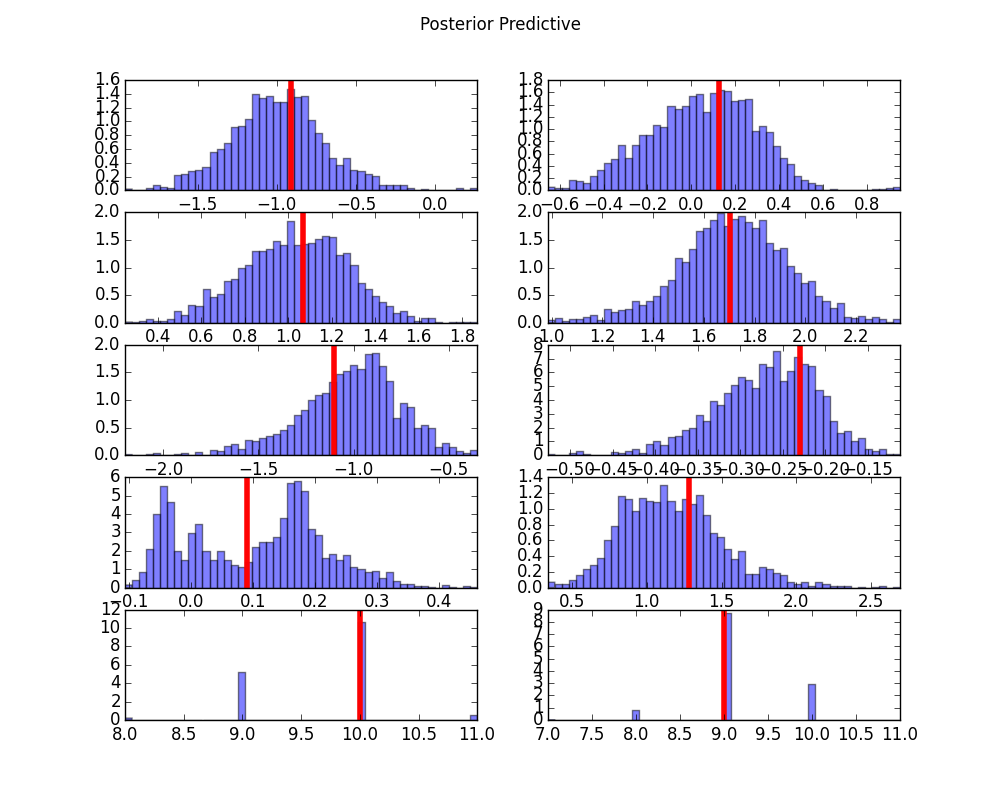
\includegraphics[width=0.45\columnwidth]{./images/blowfly_adam_postpred_sgld5k.png}
% 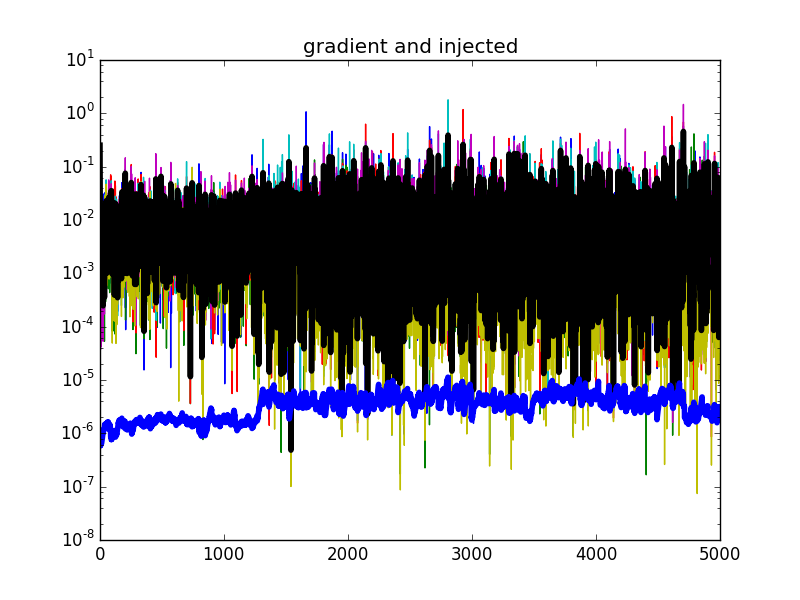
\includegraphics[width=0.45\columnwidth]{./images/blowfly_adam_noise.png}
% 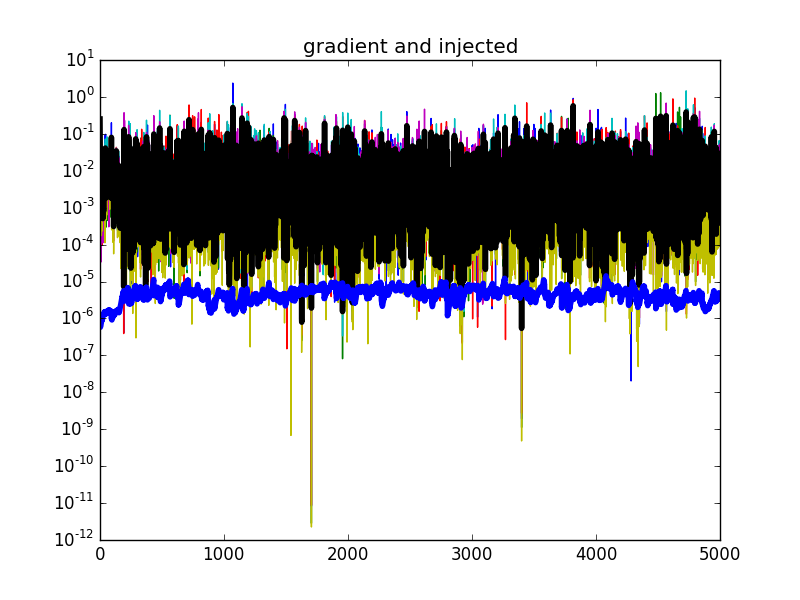
\includegraphics[width=0.45\columnwidth]{./images/blowfly_adam_noise_sgld5k.png}
% \caption{Optimizing Blowfly using $q=5$, $\epsilon = 0.01$, $\beta_1=0.75$,$\beta_2=0.9$,$\alpha=0.1$ and $c=1$.  Left: Optimization using AdaM, Right: ``SGLD'' with estimated noise. }
% \end{figure}

% \subsubsection{Using AdaM with ``SGLD" injected noise}

% \subsection{Likelihood-free Inference of Blowfly Dynamics}

% \subsection{Other Useful ABC problem}
